\subsection{Topic 5: Operating System Fundamentals -- Exercise Sheet \#1 [Solutions]}

\subsection*{Q\#1: Suppose that the processor has access to two levels of memory. Level 1 contains 1000 bytes and has an access time of 0.1\(\mu\)s; level 2 contains 100,000 bytes and has an access time of 1\(\mu\)s. Assume that if a byte to be accessed is in level 1, then the processor accesses it directly. If it is in level 2, then the byte is first transferred to level 1 and then accessed by the processor. For simplicity, we ignore the time required for the processor to determine whether the byte is in level 1 or level 2. Such a two-level memory can be shown as in figure below:}

\usetikzlibrary{shapes, arrows.meta}
\begin{center}
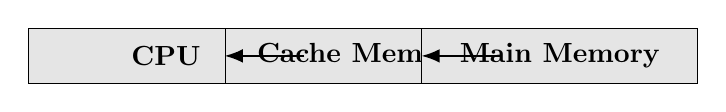
\begin{tikzpicture}[node distance=2.5cm, every node/.style={font=\bfseries}, >=Latex]
  % Define styles
  \tikzstyle{block} = [rectangle, draw=black, fill=gray!20, minimum height=2em, minimum width=3.5cm, text centered]

  % Nodes
  \node[block] (cpu) {CPU};
  \node[block, right of=cpu] (cache) {Cache Memory};
  \node[block, right of=cache] (main) {Main Memory};

  % Arrows
  \draw[->, thick] (cpu) -- (cache);
  \draw[->, thick] (cache) -- (main);
\end{tikzpicture}
\end{center}

We can define hit-ratio H, as the fraction of all memory accesses that are found in the faster memory (e.g. the cache memory). T1 is the access time to level 1 (cache) and T2 is the access time to level 2 (main memory). Now suppose 95\% of the memory accesses are found in the cache (H=0.95). Then what would be the average time to access a byte from such a two-level memory sub-system? Hint, the graph below shows the average access time to a two-level memory as a function of the hit-ratio H.

\begin{center}
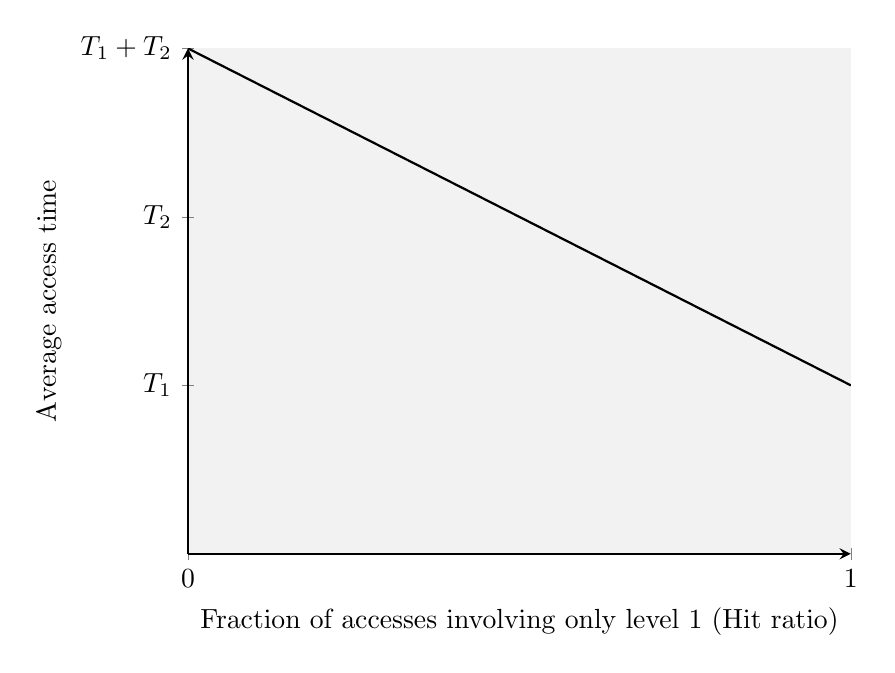
\begin{tikzpicture}
  \begin{axis}[
    width=10cm,
    height=8cm,
    xmin=0, xmax=1,
    ymin=0.5, ymax=2.0,
    axis background/.style={fill=gray!10},
    xlabel={Fraction of accesses involving only level 1 (Hit ratio)},
    ylabel={Average access time},
    xtick={0,1},
    ytick={1,1.5,2},
    yticklabels={$T_1$, $T_2$, $T_1 + T_2$},
    enlargelimits=false,
    axis lines=left,
    domain=0:1,
    samples=2,
    thick
  ]
    \addplot[black] {2 - x};  % Linear decrease from T1+T2 to T1
  \end{axis}
\end{tikzpicture}
\end{center}

\[\text{T}_{\text{Avg}} = \text{Hit Rate} \times \text{Cache access time} + \text{Miss Rate} \times \text{Lower-level access time}\]
\[
\text{T}_{\text{Avg}} = H \times T_1 + (1 - H) \times (T_1 + T_2)
\]
\[
\text{T}_{\text{avg}} = 0.95 \times 0.1\mu s + 0.05 \times (0.1\mu s + 1\mu s) = 0.095 + 0.055 = \mathbf{0.15\mu s}
\]

\subsection*{Q\#2: Consider a processor with 2 levels of memory, Level 1 Cache and Level 2 Main Memory (RAM), represented in the figure below.}

Level 1 has an access time of 11 ns and Level 2 has an access time of 0.18\(\mu s\). Assume that if a byte to be accessed is in level 1, then the processor accesses it directly. If it is in level 2, then the byte is first transferred to level 1 and then accessed by the processor. For simplicity, we ignore the time required for the processor to determine whether the byte is in level 1 or level 2.

We can define hit-ratio H, as the fraction of all memory accesses that are found in the faster memory (the cache memory). The hit-ratio H of cache is 96\%. What is the average time to access a byte in such a two-level memory subsystem?

Tavg = H * T1 + (1 - H) * (T1 + T2)
T1 = 11ns, T2 = 0.18\(\mu\)s = 180ns, H = 0.96
Tavg = 0.96 * 11 + 0.04 * (11 + 180)
Tavg = 10.56 + 0.04 * 191 = 10.56 + 7.64 = 18.2ns

\subsection*{Q\#3: A computer system has a cache, main memory, and a disk used for virtual memory. If a referenced word is in the cache, 30ns are required to access it. If it is in the main memory but not in cache, 70ns are needed to load it into cache (this includes the time to originally check the cache), and then the reference is started again. If the word is not in main memory, 10ms are required to fetch the word from disk, followed by 70ns to copy it to the cache, and then the reference is started again. The cache hit-ratio is 0.9 and the main memory hit-ratio is 0.6. What is the average time in ns required to access a referenced word on this system? }

\begin{tabular}{|l|c|c|}
\hline
\textbf{Location of the Referenced Word} & \textbf{Probability} & \textbf{Total Access Time (ns)} \\
\hline
In Cache & 0.9 & 30 \\
\hline
Not in Cache, but in Main Memory & 0.1 * 0.6 = 0.06 & 70 + 30 = 100 \\
\hline
Not in Cache or Main Memory & 0.1 * 0.4 = 0.04 & 10,000,000 + 70 + 30 = 10,000,100 \\
\hline
\end{tabular}

Average access time = (0.9 * 30) + (0.06 * 100) + (0.04 * 10,000,100)
= 27 + 6 + 400,004 = 400,037 ns

\subsection*{Q\#4: Assuming that a CPU is operating at 1 MHz, and is able to execute one instruction / clock cycle by taking benefit of pipelining. You can assume that the processor does not undertake any data read/write operations and only fetches (reads) instructions from memory.}

The DMA module on the same system is transferring characters (one byte at a time) to the main memory from an external device transmitting at 9600 bits per second. By approximately how much the processor will be slowed down due to the DMA activity?\\
1 MHz = 1 instruction/\(\mu\)s\\
DMA = 9600 bits/sec = 1200 bytes/sec\\
1 byte every 1/1200 = 833\(\mu\)s, so DMA steals 1 cycle every 833 cycles Overhead = 1 / 833 = 0.0012 = 0.12\%

\subsection*{Q\#5: We have stressed the need for an operating system to make efficient use of the computing hardware. When is it appropriate for the operating system to forsake this principle and to “waste” resources? Why is such a system not really wasteful?}
Resource usage can be justified if it enhances user experience, reliability, or functionality.

Examples:
- Keeping GUI responsive
- Keeping unused apps in memory
- Logging and monitoring
- Background updates
- Debugging

Such activities use resources but improve overall experience and safety.

\subsection*{Q\#6: What is the basic idea behind the separation between kernel mode and user mode in an operating system? How does it provide basic protection?}

Operating system uses 2 modes:
- kernel mode (privileged)
- user mode (restricted)

Protection:
- prevent user code accessing hardware/critical areas directly
- system call requests service from kernel
- system switches to kernel mode
- returns to user mode after syscall
- prevents memory corruption or unstable behaviour

\subsection*{Q\#7: Which of the following instructions should be privileged?}
\begin{itemize}
  \item a) Set value of timer
  \item b) Read the clock
  \item c) Clear memory
  \item d) Issue a trap instruction
  \item e) Turn off interrupts
  \item f) Modify entries in device-status table
  \item g) Switch from user to kernel mode
  \item h) Access I/O device
\end{itemize}
The following operations need to be privileged:
\textcolor{blue}{
\begin{itemize}
  \item a) Set value of timer
  \item c) Clear memory
  \item e) Turn off interrupts
  \item f) Modify entries in device-status table
  \item h) Access I/O device
\end{itemize}
The rest can be performed in the user mode.
}

\subsection*{Q\#8: A uniprogramming operating system runs programs that on average need 10 microseconds access to the CPU and 70 microseconds access to the I/O devices. What percentage of time is the CPU remaining idle?}

Time used for accessing CPU = 10 \textmu s / 80 \textmu s = 12.5\%  \\
Time used for accessing I/O devices = 70 \textmu s / 80 \textmu s = 87.5\%

\subsection*{Q\#9: Multi-programming (or multi-tasking) enables more than a single process to apparently execute simultaneously. How is this achieved on a uniprocessor where we have only one CPU?}

\textcolor{blue}{Multi-programming is achieved on a uniprocessor by the concept of scheduling. Every process can be given a certain amount of time, called a timeslice and when the timeslice of a process is finished, the CPU scheduler switches to a different process. The ultimate goal is to keep the system responsive while really maximising the processor's ability to process.}

\subsection*{Q\#10: What is a program? and what is a process? Discuss as many differences between them as you can imagine.}

\textbf{Program:} A program is a \textbf{group of instructions} to carry out a specified task. When we execute a program that was just compiled, the OS creates a process to execute the program. Execution of the program starts via GUI mouse clicks, command line entry of its name, etc. A program is a passive entity as it resides in the secondary memory, such as the contents of a file stored on disk. One program can have several processes.\\
\textbf{Process:} A process is a \textbf{program in execution}. The term process refers to program code that has been loaded into a computer’s memory so that it can be executed by the CPU. A process can be described as an instance of a program running on a computer or as an entity that can be assigned to and executed on a processor. A program becomes a process when loaded into memory and thus is an active entity.\\

\textbf{Differences between Program and Process:}\\
\begin{tabularx}{\textwidth}{|c|X|X|}
\hline
&\textbf{Program} & \textbf{Process} \\
\hline
1. & Program contains a set of instructions designed to complete a specific task. & Process is an instance of a program. \\
\hline
2. & Program is a passive entity as it resides in the secondary memory. & Process is an active entity as it is created during execution and loaded into the main memory. \\
\hline
3. & Program exists at a single place (such as a disk) and continues to exist until it is deleted. & Process exists for a limited span of time as it gets terminated after the completion of task. \\
\hline
4. & Program does not have any resource requirement, it only requires memory space for storing the instructions. & Process has a high resource requirement, it needs resources like CPU, memory address, I/O during its lifetime. \\
\hline
5. & Program does not have any control block or context. & Process has its own control block called PCB as well as its context. \\
\hline
\end{tabularx}



